\PassOptionsToPackage{usenames,dvipsnames,table,x11names}{xcolor}
\documentclass[11pt]{article}

%------------------------------------------------------
%                Math Packages
%------------------------------------------------------

%\usepackage[intlimits]{amsmath}
\usepackage{amsmath}
\usepackage{amssymb}
\usepackage{amsthm}
%\everymath{\displaystyle}
\usepackage{siunitx} % for SI units (e.g. C, degree)
\usepackage{bm} % bold for some math symbols
\usepackage{nicefrac} % for nicer fractions sometimes
\usepackage[thinc]{esdiff} % for derivatives
\usepackage{mathtools}

%------------------------------------------------------
%                Tikz and Pgfplots
%------------------------------------------------------

\usepackage{pgfplots}
\usepackage{tkz-euclide}
\pgfplotsset{compat=1.15}
\usetikzlibrary{arrows,shadows,positioning, calc, decorations.markings, hobby, quotes, angles, decorations.pathreplacing, intersections, matrix,backgrounds}
\usepgfplotslibrary{polar,colormaps,fillbetween}
\usepgflibrary{shapes.geometric}
%\usetkzobj{all}

%------------------------------------------------------
%                Formatting
%------------------------------------------------------

% COLORS ----------------------------------------------
%\usepackage[dvipsnames, table]{xcolor}
\usepackage{xcolor}

% FIGURES ---------------------------------------------
\usepackage{graphicx} % for importing images
\usepackage{subcaption} % for making subfigures
\usepackage[textfont=it]{caption} % changing style of figures
% labelfont=bf % sometimes use this too

% PAGE LAYOUT -----------------------------------------
%\linespread{1.3} % changes line spacing

\usepackage[a4paper, portrait, margin=1in]{geometry} % for changing layout of document
%\usepackage[a4paper, portrait, left=0.75in, right = 0.75in, top = 1in, bottom=1in]{geometry}

%\usepackage{indentfirst}
%\usepackage{parskip} % for not indenting paragraphs first
\usepackage{multirow} % having multiple rows
\usepackage{multicol} % having multiple columns
\renewcommand\labelitemi{$\vcenter{\hbox{\tiny$\bullet$}}$} % making bullets in \enumerate smaller
\usepackage[T1]{fontenc} % can combine \sc and \bf font
\usepackage{pdflscape} % for changing page orientation
\usepackage{afterpage} % to not have landscape page breaks
\usepackage{rotating} % rotating images in landscape

% LINKS -----------------------------------------------
\usepackage{etoolbox}
\makeatletter % <================================================
\patchcmd{\maketitle}%
  {\def\@makefnmark{\rlap{\@textsuperscript{\normalfont\@thefnmark}}}}%
  {\def\@makefnmark{\rlap{\@textsuperscript{\normalfont\color{blue}\@thefnmark}}}}%
  {}%success
  {}%failure
\makeatother % <=================================================
% for changing color of \thanks{} in title

\usepackage[hidelinks]{hyperref}
\hypersetup{
    colorlinks=true,
    linkcolor=black,
    filecolor=magenta,      
    urlcolor=black,
    citecolor=Blue4,
}

% LANGUAGES -------------------------------------------
\usepackage[english]{babel} % for correctly using english
\usepackage[utf8x]{inputenc} % compiling correctly
\usepackage{CJK} % using Chinese, Japanese, and Korean

% MISC ------------------------------------------------
\usepackage[normalem]{ulem} % for \sout
\usepackage{tikzsymbols} % for emojis
\usepackage{booktabs,eqparbox} % for tables
\usepackage{tabularx} % more customizable tables
\usepackage{verbatim} % for verbatim environment
%\usepackage{xmpmulti} % for animations
\usepackage{media9} % for animations

% CITING ----------------------------------------------
\usepackage{apacite}
\newcommand{\citeay}[1]{\citeauthor{#1} \citeyear{#1}}

%------------------------------------------------------
%                Custom Commands
%------------------------------------------------------

\newcommand{\done}{\hfill $\square$}
\newcommand{\csch}{\mathrm{csch}}
\newcommand{\sech}{\mathrm{sech}}

%\newcommand{\dd}{\mathop{}\,\mathrm{d}}
\newcommand{\dd}{\,\mathrm{d}}

% COLOR CODING -----------------------------------------------
\newcommand{\code}[1]{\textcolor{Bittersweet}{\texttt{#1}}} % using for emphasizing variables, code, etc.
\newcommand{\mydef}[1]{\textcolor{SteelBlue3}{\textit{#1}}} % defining something

% VENN DIAGRAMS ----------------------------------------------
\def\firstcircle{(90:1.75cm) circle (2.5cm)}
\def\secondcircle{(210:1.75cm) circle (2.5cm)}
\def\thirdcircle{(330:1.75cm) circle (2.5cm)}
\def\sampspace{(-6,-4.25) rectangle (6,5)}  %Cartesian
%\def\sampspace{(225:7cm) rectangle (45:7cm)} %polar

% TO DO LIST -------------------------------------------------
\usepackage{enumitem}

\newlist{todolist}{itemize}{2}
\setlist[todolist]{label=$\square$}

\usepackage{pifont}
\newcommand{\cmark}{\ding{51}}%
\newcommand{\xmark}{\ding{55}}%
\newcommand{\fin}{\rlap{$\square$}{\raisebox{2pt}{\color{Green}{\large\hspace{1pt}\cmark}}}%
\hspace{-2.5pt}}
\newcommand{\wontfix}{\rlap{$\square$}{\color{red}{\large\hspace{1pt}\xmark}}}

% LADE STUFF -------------------------------------------------
\xdef\defsize{4}
\xdef\cursize{5}
\newcommand{\myscale}[1]{\defsize/#1}

%------------------------------------------------------
%                Custom Environments
%------------------------------------------------------

\usepackage{mdframed}

% EXERCISE -------------------------------------------------
\mdfdefinestyle{exercise}{
	backgroundcolor=black!10,roundcorner=8pt,hidealllines=true,nobreak
}

%\begin{mdframed}[style=exercise]
%\end{mdframed}

% MATHEMATICA ------------------------------------------------
\mdfdefinestyle{mathematica}{
	backgroundcolor=Tan!15,roundcorner=8pt,hidealllines=true,nobreak,fontcolor=Bittersweet
}

% R ---------------------------------------------------------
\mdfdefinestyle{R}{
	backgroundcolor=SteelBlue3!10, roundcorner=8pt, hidealllines=true, fontcolor=SteelBlue4
}

% R ---------------------------------------------------------
\mdfdefinestyle{python}{
	backgroundcolor=Green!15, roundcorner=8pt, hidealllines=true, fontcolor=Green
}

%------------------------------------------------------
%                      Layout
%------------------------------------------------------

% FORMATTING TITLES -----------------------------------
\usepackage{titlesec}
\titleformat*{\section}{\Large \bfseries} % changing section format
\titleformat*{\subsection}{%\color{SteelBlue3} 
\large \bf} % changing subsection format
%\setcounter{secnumdepth}{0} % sets title counter to 0

% PAGE HEADINGS ----------------------------------------------
\usepackage{fancyhdr}

\pagestyle{plain}
\fancyhf{}
\lhead{}
\chead{}
\rhead{}
\cfoot{\thepage}

\renewcommand{\headrulewidth}{0.2pt}
\renewcommand{\footrulewidth}{0pt}
%\pagenumbering{gobble}

%%%%%%%%%%%%%%%%%%%%%%%%%%%%%%%%%%%%%%%%%%%%%%%%%%%%%%%
%%%%%%%%%%%%%%%%%%%%%%%%%%%%%%%%%%%%%%%%%%%%%%%%%%%%%%%
\begin{document}

%------------------------------------------------------
%                       Title
%------------------------------------------------------

\title{Sparse regression with clustered predictors}
\author{Aiden Kenny, Danielle Solomon, and Kumer Das\\
Department of Mathematics\\
Lamar University}
\date{January 24, 2020}
\maketitle

%------------------------------------------------------
%                      Document
%------------------------------------------------------

\begin{abstract}

%Gene expression data can be difficult to analyze due to its high-dimensional nature. Regularization techniques are useful in reducing the amount of predictors and highlighting the significant genes, in this case genes that may indicate the presence of cancer. The goal of this study is to see if grouping the genes before applying the regularization techniques is beneficial in reducing the prediction error of classification. We test these regularization techniques on data that has been clustered using K-means clustering and hierarchical clustering. -Stuff about the results-

%We explore the potential effectiveness of using clustering methods on high-dimensional data to improve prediction accuracy and model interpretability. Two real-world genomic data sets are used, as well as a simulation study. 

We investigate the potential effectiveness of using clustering algorithms to generate a grouping structure for high-dimensional data sets. Using various regularization techniques, we seek to determine if the generated groups are truly relevant to the response and if the accuracy and interpretability of the models can be improved. We apply the clustered group structure to two real-world data sets.

\end{abstract}

\section{Introduction}

% drawbacks to not taking advantage of group structure
% talk about why regularization is effective in high dimension, benefits over subset selection

% bc of computational ease and interpretability, in high dimension, simple models that are heavily regularized often better than more complex models (2009 paper, ESL chp 18)

% if groups are misrepresented or poorly specified, group lasso will perform poorly!

% maybe look into using group bridge instead of SGL

% both lasso and group lasso heavily shrink large coefficients and do not give consistent results (elastic net helps to abbreviate this issue)

% lambda does not have to be the same for every predictor. Say this in section 2, but then say that we assume it is the same in this paper

% maybe we should go with grpreg package and ditch gglasso and SGL, grpreg has a vast amount of models that can be fit and is computationally much much faster

% group bridge and group MCP, can both be done using grpreg package
   
%High-dimensional data sets, ones where the number of predictors vastly outnumber the number of observations, present several problems during analysis. It is difficult to take into account the influence of each of the predictors due to the exorbitant amount, and it is often the case that many of the predictors are highly-correlated. From this large pool of predictors, some predictors are more influential than others. Regularization is a useful technique when working with high-dimensional data sets; it aims to introduce a small amount of bias in the model with the hopes of drastically lowering the variance, thus improving prediction accuracy.

%Various regression models (e.g. linear and logistic) can be modified by many kinds of penalties which allow different types of regularization to occur. Genome data is an example of real-world data that is used to test these regularization techniques because of its high-dimensional nature. The lasso \cite{tibshirani1996regression} minimizes the loss function with an added $\ell_1$ penalty imposed on the coefficient vector $\bm{\beta}$. If the shrinkage is severe enough, entire coefficients will be set to zero, i.e. the lasso produces \textit{sparse} models. However, there are times when the lasso does not perform well (e.g. when the predictors are highly-correlated); one alternative is the \textit{elastic net} \cite{zou2005regularization}, which imposes a combination of an $\ell_1$ penalty and a squared $\ell_2$ penalty. 

%One drawback of the lasso is that it does not take into account any grouping structure within the data, which can often be exploited to improve prediction accuracy. The group lasso (gLasso) \cite{yuan2006model} imposes an $\ell_2$ norm on each of the pre-defined groups. As a result, gLasso imposes sparsity \textit{among} different groups; however, one drawback is that there is no sparsity \textit{within} each group. A compromise is the sparse group lasso (sgLasso) \cite{friedman2010note} combines the lasso and gLasso penalties, and the resulting model will have sparsity both within and among the groups. %This is especially useful in regards to genome data because sparse group lasso is useful in identifying the pathways of interest and and selecting pathways of interest from them. 
%Sparse group lasso also shrinks the estimated effects of driving genes within a group toward one another (Simon et al). 

%Principal components lasso (pcLasso) \cite{2018arXiv181004651T} is another method that can be applied both without and with group structure. It applies both an $\ell_1$ penalty on the entire coefficient vector and a ``pcLasso penalty'' to each group. The pcLasso penalty is a quadratic penalty based off of the SVD of each group. For each group, pcLasso shrinks each group vector toward that group's leading principal axis. %PcLasso also is capable of inducing group sparsity, similar to group lasso. However, pcLasso has proven to be more equipped to handle data sets that can be too large for sparse group lasso. 

%It is often the case that the groups for a data set are known before the analysis is performed. If the data set has some type of grouping structure that is not known, this grouping structure cannot be exploited to improve prediction accuracy. It is possible to perform \textit{cluster analysis}, an unsupervised learning technique, on the data set an gain an insight on the possible group structure. We can then perform regularization using these groups as the predictors, hopefully improving prediction accuracy. 
%However, there are not many studies that cluster the data before employing these regularization techniques and use the regularization techniques on the entire data set. It is unsure if there is difference in the outcome when using that has been pre-clustered versus data that is considered as a whole. We are going to compare the prediction accuracy of these different regularization techniques applied to a data set as a whole versus the clustered version of the same data set.

%We want to see if applying unsupervised clustering methods to data sets has the ability to improve prediction accuracy. 

The idea of using data and information to train models that are both accurate and interpretable has been around for decades. One desires to build a model based on the \textit{predictors} that is both accurate and interpretable; we want our models to correctly predict the outcome and we want to know which predictors are responsible. However, in the age of big data it is becoming increasingly common that a data set is \textit{high-dimensional}, meaning the number of predictors $p$ vastly exceeds the number of observations $n$. In this setting, many longstanding statistical modeling techniques, such as linear and logistic regression, no longer suffice. Regularization is a popular technique that imposes a penalty on the original model; in some cases the models are \textit{sparse}, meaning they are very interpretable.

It is sometimes the case that the predictors of a model belong to some kind of pre-defined group, and the response is now based on these groups, as opposed to the individual predictors. More advanced regularization methods have been developed to accommodate for group structure, and assuming that the groups are well-represented, can greatly improve the accuracy and interpretability of the models. Unfortunately, while the response could truly be dependent on the group structure, the actual grouping structure is unknown beforehand. In this situation, one would desire to properly identify the grouping structure and build a model based on the result.

The goal of this paper is to investigate the effect that clustering can have on regularized models. We seek to answer two questions:
\begin{enumerate}
    \item Can clustering algorithms be used to properly identify a grouping structure in a data set?
    \item Can grouping the predictors using the clustering information improve the accuracy and interpretability of the model?
\end{enumerate}
In Section 2 we provide a brief overview of the various regularization techniques and clustering algorithms we used in our study. Sections 3 and 4 investigate the effect of clustering predictors on two real-world genomic data sets, and we close with a discussion in Section 5.

\section{Methodology}

\subsection{Logistic regression}

In many situations, the response variable of a data set is categorical in nature, and we wish to assign an observation to one of the response variables given its inputs, a process known as classification. We seek to model the \textit{probability} that an observation falls into a given class. It is often the case where the response belongs to one of two classes coded as $\mathcal{G} = \{ 0,1 \}$. In this binary setting, one popular approach to modeling the probabilities is \textit{logistic regression}.

Suppose we have $n$ observations and $p$ predictors stored in a data matrix $\mathbf{X} = \{ x_{i,j} \}$ for $i = 1, \ldots, n$ and $j = 1, \ldots, p$, along with a response vector $\mathbf{y} = (y_1, \ldots, y_n)$, where $y_i \in \{ 0,1 \}$. If $p(\bm{x}_i) = \mathbb{P}(Y = 1 \mid X = \bm{x}_i)$, where $\bm{x}_i = (x_{i,1}, \ldots, x_{i,p})$ is the $i$th observation in $\mathbf{X}$,
then the probability is modeled (as the log-odds) by
\begin{align}
    \label{logprob}
    \log \left( \frac{p(\bm{x}_i)}{1 - p(\bm{x}_i)} \right) = \beta_0 + \bm{x}_i^T \bm{\beta}.
\end{align}
From this, the estimated response $\hat{y}_i$ is 1 if $p(\bm{x}_i) \ge 0.5$ and 0 otherwise. The coefficients $\beta_0$ and $\bm{\beta} = (\beta_1, \ldots, \beta_p)$ are estimated from the data by minimizing the negative log-likelihood function
\begin{align}
\label{negloglike}
    L (\beta_0, \bm{\beta}) = \frac{1}{n} \sum_{i = 1}^n \Big[ \log \left(1 + e^{\beta_0 + \bm{x}_i^T \bm{\beta}}  \right)  - y_i \big(\beta_0 + \bm{x}_i^T \bm{\beta} \big)\Big].
\end{align}
%That is, $(\hat{\beta}_0 , \hat{\bm{\beta}}) = \underset{\beta_0, \bm{\beta}}{\mathrm{argmin}} L (\beta_0, \bm{\beta})$. 
%The coefficient vector $\bm{\beta}$ can give insight to the effect that each %predictor has on the response. If $\hat{\beta}_j = 0$, then we infer that the $j$th predictor does not have an effect on the response. This interpretability is one advantage that logistic regression has over other classification methods, such as linear discriminant analysis (LDA) or K-nearest neighbors (KNN). 

\subsection{Basic regularization}

%high dim data, big data, often we don't know which predictors to use. If try to fit all, bad (explain why), regularization helps with this. Introduce methods

% explain high-dimensional setting
%Statistical modeling has traditionally consisted of predicting a response based off of relatively few predictors, where these important predictors are determined from domain expertise. However, in the age of big data, it is increasingly the case that we want to make predictions using high-dimensional data, where the number of predictors is much larger than the number of observations, i.e. $p \gg n$. Many difficulties arise in this situation, and basic statistical methods, including logistic regression, prove to no longer be sufficient models.

%Regularization involves fitting a linear model with all possible predictors while imposing some type of penalty on the coefficient vector $\bm{\beta}$. In the high-dimensional setting these highly-regularized linear models are favorable, as they are simple yet provide vast improvements in both prediction accuracy and interpretability. Regularization can be applied to many different types of models, but for this paper we focus on its application to logistic regression.

% this stuff is all good for introduction

In general, a regularized linear model seeks to minimize a penalized version of (\ref{negloglike}) of the form
\begin{align*}
    Q(\beta_0, \bm{\beta}) = L(\beta_0, \bm{\beta}) + \lambda P(\bm{\beta}),
\end{align*}
where $P(\bm{\beta})$ is some type of penalty imposed on the coefficient vector $\bm{\beta}$. The tuning parameter $\lambda \ge 0$ effectively controls the severity of the penalty; as the value of $\lambda$ increases, more shrinkage is imposed on the coefficients. 

Various regularization methods have been introduced throughout the years using different penalty functions, with each method shrinking the coefficients in a different way. \textit{Ridge regression} \cite{hoerl1970ridge} imposes a squared $\ell_2$ norm on $\bm{\beta}$, and seeks to minimize 
\begin{align}
    \label{ridgeregression}
    Q(\beta_0, \bm{\beta}) = L(\beta_0, \bm{\beta}) + \frac{\lambda}{2} \| \bm{\beta} \|_2^2.
\end{align}
The $\ell_2$ norm causes continuous shrinkage of the estimated coefficients. %Ridge regression improves prediction accuracy over the ordinary logistic regression model due to the bias-variance trade-off. 
A major drawback to ridge regression is that it produces dense models, i.e. models where $\beta_j \not = 0$ for all $j$, an undesirable characteristic for an interpretable model.

An alternative similar to ridge regression is the \textit{lasso} \cite{tibshirani1996regression}, which minimizes 
\begin{align}
    \label{lasso}
    Q(\beta_0, \bm{\beta}) = L(\beta_0, \bm{\beta}) + \lambda \| \bm{\beta} \|_1.
\end{align}
Here, an $\ell_1$ norm is imposed on $\bm{\beta}$, as opposed to a squared $\ell_2$ norm. Unlike ridge regression, the lasso is able to perform variable selection, forcibly setting many estimated coefficients to zero, producing sparse models. %This feature makes the lasso extremely desirable in high-dimensional settings, as the resulting models are interpretable, and is often preferred over ridge regression for this reason.
The resulting sparsity of the model often makes the lasso more preferable than ridge regression in the high-dimensional setting. Unfortunately, the lasso has several caveats as well; in the high-dimensional setting the lasso will select at most $n$ predictors, and if several predictors are highly-correlated, the lasso will select only one and force the others to zero. 

A generalization to ridge regression and the lasso, which attempts to combine the benefits while negating the drawbacks, is the \textit{elastic net}\footnote{\citeay{zou2005regularization} call this penalty the \textit{na\"{i}ve} elastic net penalty, and suggest that scaling the estimated coefficients up by a factor of $1 + \lambda(1 - \alpha)$ improves prediction accuracy. However, in their paper describing the implementation of the elastic net, \citeay{friedman2010regularization} abandon this distinction.} \cite{zou2005regularization}, which minimizes
\begin{align}
    \label{elasticnet}
    Q(\beta_0, \bm{\beta}) = L(\beta_0, \bm{\beta})
    + \lambda \Big[ \alpha \| \bm{\beta} \|_{1} + \frac{1 - \alpha}{2} \|\bm{\beta}\|_{2}^{2} \Big].
\end{align}
This penalty is a linear combination of (\ref{ridgeregression}) and (\ref{lasso}), and the mixing parameter $\alpha \in [0,1]$ is used to determine how much of each type of penalty is imposed on the model; $\alpha = 0$ corresponds to ridge regression, while $\alpha = 1$ gives the lasso. 

\subsection{The group setting}

%It is often the case that many predictors in a data set are not distinct, and instead belong to some kind of group. A specific example is gene expression data, where the genes can be grouped by their pathways. In this situation, methods that perform individual variable selection, such as the lasso, will often perform poorly due to their inability to exploit information from the grouping structure. In addition, one may wish to know which groups are important to the response, in addition to the individual predictors. 
%\citeay{zou2005regularization} show that the elastic net has the ability to exploit group structure in the data, something that neither ridge regression nor the lasso can do. However, this exploitation comes from the predictors having some type of strong correlation, as opposed to some kind of pre-determined grouping structure. 

Much work has been done to develop penalties that exploit pre-determined group structure. Suppose that the predictors of $\mathbf{X}$ are split into $K$ non-overlapping groups, with $S_k$ denoting the size of the $k$th group. For $k = 1, \ldots, K$, let $\mathbf{X}_k \in \mathbb{R}^{n \times S_k}$ denote the data matrix with the predictors in group $k$, and let $\bm{\beta}_k = (\beta_{k,1}, \ldots, \beta_{k, S_k})$ be the sub-vector of $\bm{\beta}$ corresponding to the $k$th group. 

The \textit{group lasso} (``gLasso'') \cite{yuan2006model} imposes an $\ell_2$ norm on each of the coefficient sub-vectors; it minimizes 
\begin{align}
    \label{grouplasso}
    Q(\beta_0, \bm{\beta}) = L(\beta_0, \beta) + \lambda \sum_{k=1}^K \sqrt{S_k} \| \bm{\beta}_k \|_2.
\end{align}
The group lasso was later extended to logistic regression by \citeay{meier2008group}. The $\ell_2$ penalties on each of the coefficient sub-vectors creates sparsity among the different groups while performing ridge shrinkage within each group. %In the special case of $S_k = 1$ for all $k$, i.e. there is no grouping structure, the group lasso becomes the lasso, so the group lasso can be thought of as a type of generalization of the lasso.
As a result, the group lasso unfortunately only induces sparsity at the group level, and if a group is determined to be significant, \textit{all} of the group's predictors will be nonzero.

Both \citeay{yuan2006model} and \citeay{meier2008group} assume that the data is orthonormal within each group, i.e. $\mathbf{X}_k^T \mathbf{X}_k = \mathbf{I}$ for all $k$. This is almost never the case in practice, so one would want to orthonormalize each $\mathbf{X}_k$ before minimizing (\ref{grouplasso}). However, as \citeay{simon2012standardization} show, this actually changes the penalty to
\begin{align}
    \label{altgrouplasso}
    Q(\beta_0, \bm{\beta}) = L(\beta_0, \beta) + \lambda \sum_{k=1}^K \sqrt{S_k} \| \mathbf{X}_k \bm{\beta}_k \|_2.
\end{align}
This alternative penalty is theoretically and computationally superior \cite{breheny2015group} to (\ref{grouplasso}), so for the rest of this paper we refer to (\ref{altgrouplasso}) when speaking about the group lasso. 

%As mentioned before, the group lasso only produces sparsity among the different groups, not within them; for a given group, either all of the group's coefficients are set to 0, or none of them are. This presents a major problem for model interpretability, as one may wish to determine the significant predictors within each group. In addition, the group lasso is biased, as it heavily shrinks large groups. 

There are several methods used in practice to induce sparsity both within and among groups, a feature known as \textit{bi-variate selection}. 
%such as the \textit{sparse group lasso} \cite{simon2013sparse} and the \textit{group bridge} \cite{huang2009group}. 
One method is to combine the lasso and the group lasso penalties as a linear combination, similar to the elastic net; the resulting penalty is known as the the \textit{sparse group lasso} \cite{simon2013sparse}, and minimizes 
\begin{align}
    \label{sparsegrouplasso}
    Q(\beta_0, \bm{\beta}) = L(\beta_0, \bm{\beta}) + \lambda \left[ \alpha \| \bm{\beta} \|_1 + (1 - \alpha) \sum_{k=1}^K \sqrt{S_k}  \| \bm{\beta}_k \|_2 \right].
\end{align}
With this penalty, sparsity is induced at the group level, and elastic net-type shrinkage is imposed within each group. Unfortunately, unlike the group lasso, there is no way to orthonormalize each group without corrupting the within-group sparsity effect, making any implementation of the sparse group lasso difficult compared to other penalties.

An alternative method for performing bi-variate selection is the \textit{composite minimax concave penalty}\footnote{\citeay{breheny2009penalized} originally denote cMCP as the \textit{group} MCP. To avoid confusion, \citeay{huang2012selective} recommend denoting (\ref{cMCP}) as the \textit{composite} MCP.} (``cMCP'') \cite{breheny2009penalized}, which minimizes
\begin{align}
    \label{cMCP}
    Q(\beta_0, \bm{\beta}) = L(\beta_0, \bm{\beta}) + \sum_{k=1}^K f_{\lambda, \Gamma_k} \left( \sum_{s=1}^{S_k} f_{\lambda, \gamma}(|\beta_{k,s}|) \right).
\end{align}
Here $f_{\lambda, \gamma}(\cdot)$ is the minimax concave penalty \cite{zhang2007penalized}, given by 
\begin{align}
    \label{MCPpenalty}
    f_{\lambda, \gamma}(\phi) = \begin{cases}
        \lambda \phi - \frac{\phi^2}{2 \gamma}, & \text{if } \phi \le \gamma \lambda \\
        \frac{1}{2} \gamma \lambda^2, & \text{if } \phi > \gamma \lambda
    \end{cases}.
\end{align}
The intuition behind (\ref{MCPpenalty}) is to counter the aggressive shrinkage that the lasso imposes on large coefficients. The parameter $\gamma > 0$ controls the ``range'' of this counter, and the penalty becomes the lasso as $\gamma \to \infty$. We can see that (\ref{cMCP}) is effectively applying the penalty twice, once to induce sparsity within each group and then again to induce sparsity among the groups. The outer parameter is set to $\Gamma_k = \frac{1}{2} S_k \gamma \lambda$, while the inner penalty $\gamma$ is the same throughout. 


%In addition to $\lambda$, we have two additional parameters $\Gamma_k$ and $\gamma$, the former controlling the range of the outer penalty and the latter controlling the range of the inner penalty. In order to assure that the group level penalty attains its maximum value, we always choose $\Gamma_k = \frac{1}{2} S_k \gamma \lambda$. The choice of $\gamma$ will depend on the situation; for logistic regression, \citeay{breheny2009penalized} recommend using $\gamma = 30$, since the response variable is always on the same scale (either 0 or 1). 

% find part in paper that talks about adding ell2 norm to this

\subsection{Regularization based on principal components}

Let $\mathbf{X} = \mathbf{U} \mathbf{D} \mathbf{V}^T$ be the singular value decomposition of the data matrix, and let $m = \mathrm{rank}(\mathbf{X})$. The principal axes, or right singular vectors, are given by the columns of $\mathbf{V} \in \mathbb{R}^{p \times m}$, and $\bm{d} = (d_1, \ldots, d_m)$ are the singular values such that $d_1 \ge \ldots \ge d_m > 0$. $\mathbf{D} \in \mathbb{R}^{m \times m}$ is a diagonal matrix whose diagonal entries are the elements of $\bm{d}$. 

Principal components lasso (``pcLasso'') \cite{2018arXiv181004651T} minimizes 
\begin{align}
    \label{pcLasso}
    Q(\beta_0, \bm{\beta}) = L(\beta_0, \bm{\beta}) + \lambda \| \bm{\beta} \|_1 + \frac{\theta}{2} \bm{\beta}^T \Big( \mathbf{V} \mathbf{D}_{d_1^2 - d_j^2} \mathbf{V}^T \Big) \bm{\beta},
\end{align}
where $\lambda$ and $\theta$ are two separate tuning parameters. The diagonal matrix $\mathbf{D}_{d_1^2 - d_j^2} \in \mathbb{R}^{m \times m}$ has diagonal inputs that are functions of the singular values of $\mathbf{X}$, and is given by 
\begin{align}
    \label{pcLassopenaltymatrix}
    \mathbf{D}_{d_1^2 - d_j^2} = \mathrm{diag}(d_1^2 - d_1^2, d_1^2 - d_2^2, \ldots, d_1^2 - d_m^2).
\end{align}
This ``pcLasso penalty'' has the result of imposing less shrinkage in the direction of the leading principal axis and more severe shrinkage in the directions of subsequent principal axes. In other words, $\bm{\beta}$ is biased in the direction of the leading principal axis. %By strongly biasing the coefficient vector $\bm{\beta}$ in the direction of the leading principal axis, pcLasso hopes to improve prediction accuracy. 
The presence of the $\ell_1$ norm allows pcLasso to simultaneously perform feature selection. 

pcLasso can also be modified to exploit group structure. Let $\mathbf{X}_k = \mathbf{U}_k \mathbf{D}_k \mathbf{V}_k^T$ be the singular value decomposition for the $k$th group matrix, and let $m_k = \mathrm{rank}(\mathbf{X}_k)$. Then the columns of $\mathbf{V}_k$ and $\bm{d}_k = (d_{k,1}, \ldots, d_{k, m_k})$ are the principal axes and singular values of $\mathbf{X}_k$, respectively. In this setting, pcLasso seeks to minimize
\begin{align}
    \label{pcLassogroup}
    Q(\beta_0, \bm{\beta}) = L(\beta_0, \bm{\beta}) + \lambda \| \bm{\beta} \|_1 + \frac{\theta}{2} \sum_{k=1}^K \sqrt{S_k} \bm{\beta}_k^T \Big( \mathbf{V}_k \mathbf{D}_{d_{k,1}^2 - d_{k,j}^2} \mathbf{V}_k^T \Big) \bm{\beta}_k.
\end{align}
Similar to (\ref{pcLassopenaltymatrix}), the matrix $\mathbf{D}_{d_{k,1}^2 - d_{k,j}^2} \in \mathbb{R}^{m_k \times m_k}$ is given by 
\begin{align}
    \label{pcLassopenaltymatrixgroup}
    \mathbf{D}_{d_{k,1}^2 - d_{k,j}^2} = \mathrm{diag}(d_{k,1}^2 - d_{k,1}^2, d_{k,1}^2 - d_{k,2}^2, \ldots, d_{k,1}^2 - d_{k,m_k}^2).
\end{align}
We now see that pcLasso biases each coefficient sub-vector $\bm{\beta}_k$ in the direction of that group's leading principal axis, all while producing sparse models. Unlike the group lasso and cMCP, pcLasso does not require each group matrix $\mathbf{X}_k$ to be orthonormal. 

%\citeay{2018arXiv181004651T} show that pcLasso is able to perform bi-variate selection in some situations. That is, while it will always induce sparsity among the predictors, it has the potential to induce sparsity among the groups as well. Let $\mathbf{X}_k^T \mathbf{X}_k/(n-1) = \mathbf{V}_k \mathbf{D}_k^2 \mathbf{V}_k^T/(n-1)$ be the eigendecomposition of the covariance matrix of $\mathbf{X}_k$, scaled up by a factor of $n - 1$. The $i$th eigenvalue $\lambda_i = d_i^2/(n-1)$ give the variance along the $i$th principal axis. 

% work on this

\subsection{Clustering methods}

%Clustering is an unsupervised learning technique used to gain valuable insights about a data set. 
In general, a clustering algorithm seeks to partition the predictors of a data set into different sub-groups based on some dissimilarity measure; ideally, the dissimilarity will be low for predictors within the same cluster and high for predictors in separate clusters. Various clustering algorithms and dissimilarity measures exist that seek to achieve this goal, so for this report we only focus on two simple algorithms.

\textit{$K$-means clustering} \cite{macqueen1967some} clusters the predictors into $K$ non-overlapping groups based on their Euclidean distance in the observation space. 
Let $C_k$ be the set of all predictors that belong to group $k$, for $k = 1, \ldots, K$, and let $S_k$ denote the number of predictors in group $k$. $K$-means clustering seeks to minimize the total within-cluster variation, given by 
\begin{align}
    \label{totwithinclusvar}
    W_K = \sum_{k=1}^K \sum_{j \in C_k} \| \mathbf{x}_j - \bar{\mathbf{x}}_k \|_2^2,
\end{align}
where $\mathbf{x}_j$ is the $j$th predictor and $\bar{\mathbf{x}}_k = \frac{1}{S_k} \sum_{j \in C_k} \mathbf{x}_j$ is the $k$th group centroid. %$K$-means clustering hopes to define $K$ different groups using the Euclidean distance of the predictors in the observation space; in this space, predictors close to each other will be grouped together, while predictors far away will not. %See Appendix X for a more thorough discussion on the potential performance of clustering predictors in this way.

One drawback of $K$-means clustering is that the number of clusters $K$ must be supplied before $W_K$ can be minimized. Given that we have no information about the group structure beforehand, we desire some type of measurement to determine the optimal number of clusters. %One could try to arbitrarily increase $K$ until a minimum $W_K$ is found, but it can be shown that $W_K$ will always decrease as $K \to \infty$. However, after a certain value of $K$, the rate of this decrease will be quite small, indicating that adding new clusters does not 
The GAP statistic \cite{tibshirani2001estimating}, defined as 
\begin{align}
    \label{GAPstat}
    \mathrm{Gap}(m) = \mathbb{E} \left[ \log(W_m) \right] - \log(W_m),
\end{align}
attempts to choose an optimal $K$ from the rate that $W_K$ decreases. Given a maximum amount of clusters $M$, the gap statistic is estimated using $B$ Monte Carlo random samples; the optimal number of clusters $K$ is chosen  when $\mathrm{Gap}(K) \ge \mathrm{Gap}(K + 1) - \delta(K + 1)$, where 
\begin{align*}
    \delta(m) = \mathrm{sd}_m \sqrt{1 + \frac{1}{B}}
\end{align*}
and $\mathrm{sd}_m$ is the standard deviation of the $B$ estimated $W_m$'s.

%It can be shown that $W_K$ will always decrease as $K$ increases, but at a certain point $W_K$ will start to decrease slowly; the GAP statistic identifies this cut-off point as the optimal number of clusters. See Appendix \ref{AppA} for more information about calculating $\mathrm{Gap}(K)$ and determining the optimal $K$.

Another appealing clustering algorithm is \textit{hierarchical clustering}, which groups the predictors into nested clusters. While Euclidean distance could be used as the choice of dissimilarity, we chose to use correlation instead to investigate how this choice effects the resulting group structure. Unlike $K$-means clustering, there is no criteria that could be used to choose the optimal number of clusters. Fortunately, given that the clusters are nested, they can be represented in a dendrogram where the number of clusters can be chosen by the user. 

%\newpage


%\subsection{Hierarchical Clustering}
%\emph{Hierarchical clustering} provides an alternate method of clustering data. Unlike $K$-means clustering, hierarchical clustering does not require pre-specified $k$ clusters. It results in a tree-based representation of the observations, known as a dendogram. A dendogram is constructed starting from the leaves and combining clusters up to the trunk. Each leaf of the dendogram represents an observation. When leaves begin to fuse into branches, it indicates that the observations are similar to each other. Branches can fuse with other branches or leaves when moving further up the tree. The height of the fusion indicates how similar or different the observations are. 
%Both $K$-means clustering and hierarchical clustering include all the observations in a data set. 








%\section{Real-world Examples}

%A common real world occurrence of high-dimensional data is in gene expression data. Both data sets that we are working with are cancer gene expression data. Genome data often has a group structure within the data set which is compatible with these particular regularization techniques. 
%The first data set is the colon cancer data set. The data set features 2000 genes with the highest minimal intensity across 62 tissues. Of the 62 tissue samples, 40 of them are tumorous and 22 are healthy tissues. 

%The second data set is the leukemia data set. It consists of 7128 genes from 72 patients. 

%Both of these data sets have been previously used in studies for binary classification, specifically whether or not each gene is cancerous.





\section{Colon data set}

The colon data set, originally introduced by \citeay{alon1999broad}, contains the gene expressions of 2,000 genes for 62 different tissue samples, i.e. $n = 62$ and $p = 2,000$. Of the 62 tissue samples, 40 of the samples tested positive for colon cancer, while 22 tested negative. 

\subsection{Clustering information}

\begin{figure}[ht]
    \centering
    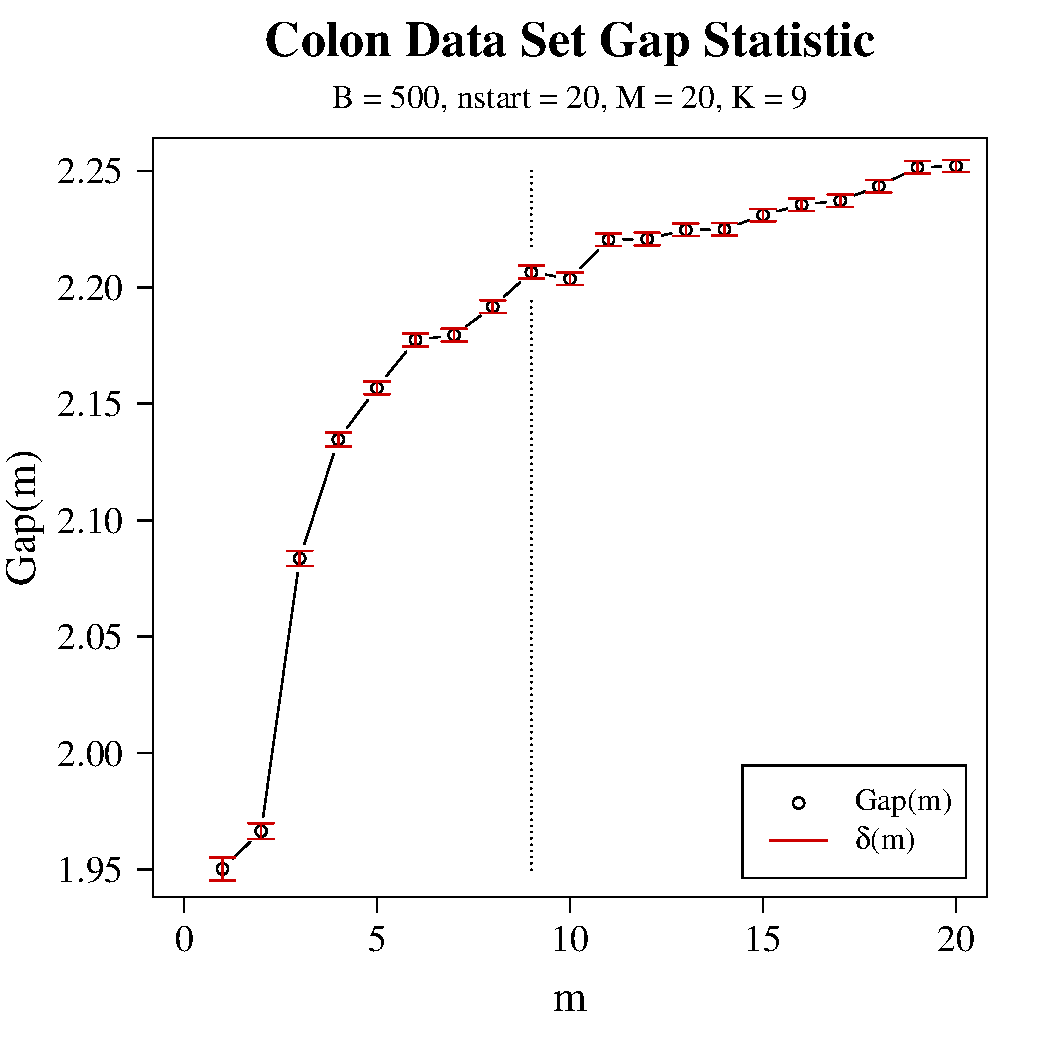
\includegraphics[width = 0.475\textwidth]{colon_gap_stat.pdf}
    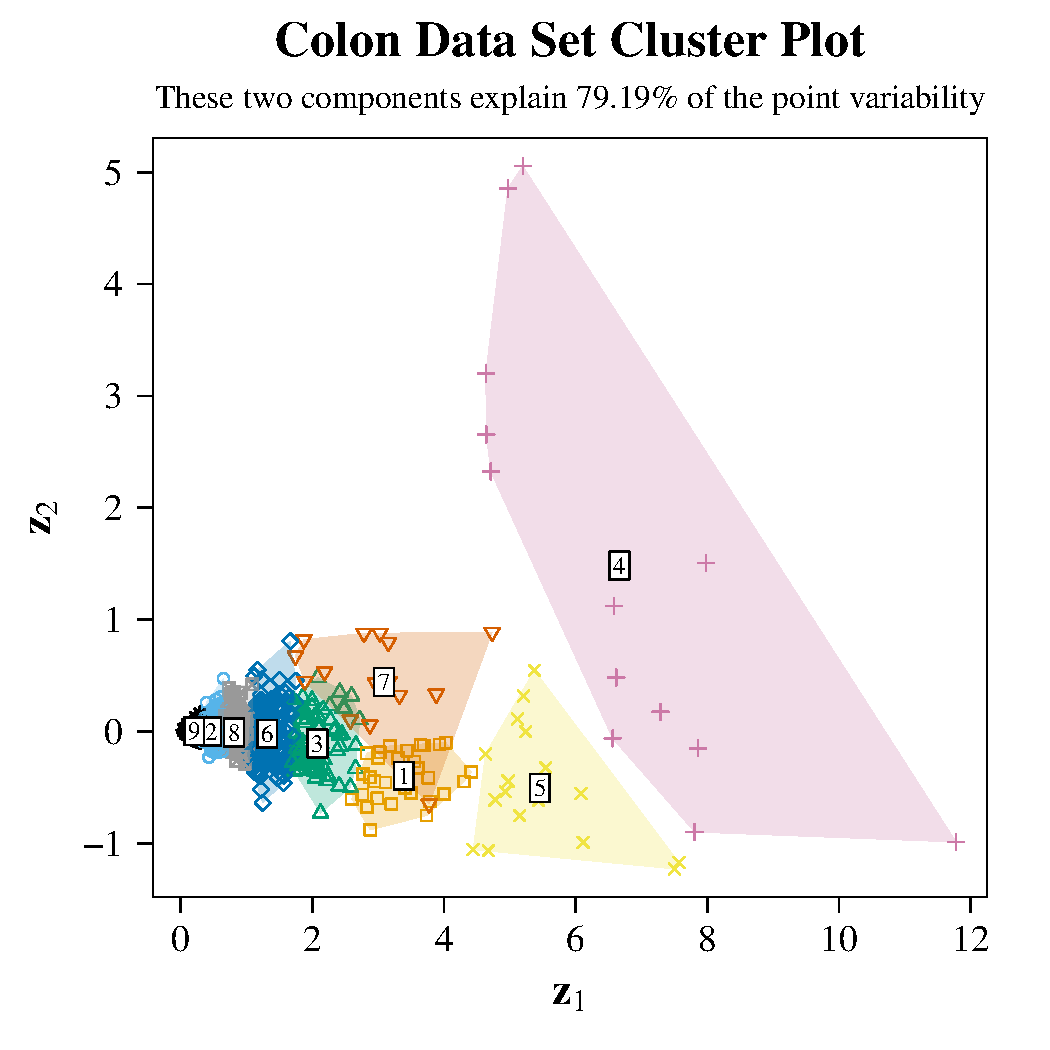
\includegraphics[width = 0.475\textwidth]{colon_clus_plot.pdf}
    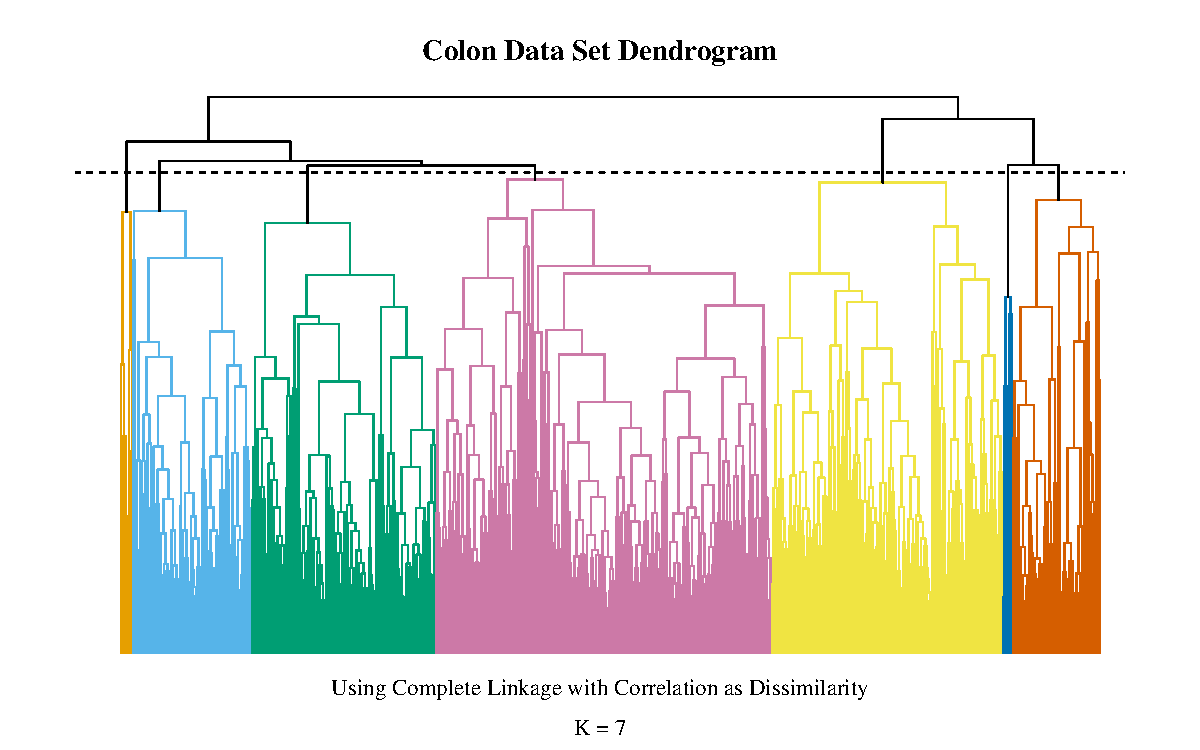
\includegraphics[width = 0.95\textwidth]{colon_den.pdf}
    \caption{Clustering information for the colon data set.}
    \label{colonclus}
\end{figure}

Figure \ref{colonclus} shows the clustering information for the colon data set. The top-left panel measures the gap statistics for $m = 1, \ldots, 20$, and chooses $K = 9$ as the optimal number of clusters using $K$-means clustering. The top-right panel plots the predictors against the first two columns of $\mathbf{Z} = \mathbf{V} \mathbf{D}$ (where $\mathbf{V} \mathbf{D} \mathbf{U}^T = \mathbf{X}^T$ is the SVD of the transposed data matrix, so the columns of $\mathbf{Z}$ are the principal components of $\mathbf{X}^T$), along with the labeled groups that each predictor belongs to. 

The bottom panel displays the corresponding dendrogram using correlation as the dissimilarity measure for hierarchical clustering. We decided that $K = 7$ was a reasonable cut-off for this dendrogram. 

\subsection{Results}

For all of the following methods, we randomly split the data set into a training set and a test set, both with 31 observations each. Each model was fit on the training set, and its performance was measured on the test set. Models that have additional parameters besides $\lambda$ were fit using a grid of values of said parameter (e.g. $\alpha$ for the elastic net), and the model with the lowest deviance was chosen. 

We first fit the following regularized models on the colon data set \textit{without} any grouping structure:
\begin{enumerate}
    \item The lasso: was fit using \texttt{glmnet} version \texttt{2.0.16}.
    \item The elastic net: was fit for $\alpha = 0.95, 0.8, 0.6, 0.4, 0.2, 0.05$, using \texttt{glmnet} version \texttt{2.0.16}.
    \item pcLasso: was fit for \texttt{rat}\footnote{As opposed to testing over a grid of values for $\theta$, \citeay{2018arXiv181004651T} suggest specifying a value of \texttt{rat} instead. More details can be found in their paper.} $= 0.95, 0.9, 0.75, 0.5, 0.25, 0.1$, using \texttt{pcLasso} version \texttt{1.1}.
\end{enumerate}
Next, we fit the following models on the colon data set using the grouping structure obtained from $K$-means clustering:
\begin{enumerate}
    \item gLasso: was fit using \texttt{grpreg} version \texttt{3.2.1}.
    \item sgLasso: was fit for $\alpha = 0.95, 0.8, 0.6, 0.4, 0.2, 0.05$, using \texttt{SGL} version \texttt{1.2}.
    \item cMCP: was fit for $\gamma = 30$, using \texttt{grpreg} version \texttt{3.2.1}.
    \item pcLasso: was fit for $\texttt{rat} = 0.95, 0.9, 0.75, 0.5, 0.25, 0.1$, using \texttt{pcLasso} version \texttt{1.1}.
\end{enumerate}
The \texttt{clusGap} function from \texttt{cluster} version \texttt{2.1.0} was used to calculate the gap statistic, and the groups were clustered using the \texttt{kmeans} function. Finally, the process above was repeated using the grouping structure from hierarchical clustering, which was obtained using the \texttt{hclust} function.

The results from the various models are presented in Table \ref{colontab}. Included in the table are the values of the optimized parameters, the cross-validation deviance, the number of missclassifications on the test set, the number of nonzero coefficients in the final model (including the intercept $\beta_0$), the number of significant groups in the final model (if a single group contained a nonzero coefficient, then it is considered significant), and the area under the curve (AUC) measurements. The corresponding ROC curves for each model have been printed in Figure \ref{colonROC}.

\afterpage{
\begin{landscape}
\begin{table}[p]
    \footnotesize
    \centering
    \def\arraystretch{1.5}

    \begin{tabularx}{0.971\linewidth}{lccccccccccc} \toprule
         & \multicolumn{3}{c}{No Clustering} & \multicolumn{4}{c}{$K$-means Clustering} & \multicolumn{4}{c}{Hierarchical Clustering} \\ 
         & \multicolumn{3}{c}{--} & \multicolumn{4}{c}{$K=9$} & \multicolumn{4}{c}{$K=7$} \\   
         \cmidrule(r){2-4} \cmidrule(lr){5-8} \cmidrule(l){9-12}
         % this is what has to be replaced with xtable
         & Lasso & Elastic Net & pcLasso & gLasso & sgLasso & cMCP & pcLasso & gLasso & sgLasso & cMCP & pcLasso \\ \midrule
        \multirow{2}{*}{Parameters} & $\lambda = 0.0642$ & $\lambda = 0.0853$ & $\lambda = 8.75$ & $\lambda = 0.00562$ & $\lambda = 0.0215$ & $\lambda = 0.0838$ & $\lambda = 35.32$ & $\lambda = 0.0621$ & $\lambda = 0.0194$ & $\lambda = 0.0813$ & $\lambda = 163.94$ \\ 
        & -- & $\alpha = 0.95$ &  $\texttt{rat} = 0.95$ & -- & $\alpha = 0.4$ & $\gamma = 30$ & $\texttt{rat} = 0.25$ & -- &  $\alpha = 0.05$ & $\gamma = 30$ & $\texttt{rat} = 0.95$ \\ 
        Deviance & 0.938 & 0.945 & 0.561 & 0.490 & 0.853 & 1.01 & 0.525 & 0.987 & 0.863 & 0.995 & 0.548 \\ 
        Misclass. & 6/31 & 6/31 & 5/31 & 12/31 & 7/31 & 6/31 & 5/31 & 8/31 & 11/31 & 6/31 & 3/31 \\ 
        Sig. Coef. &  16 &  19 &  30 &  49 &  29 &  11 &  30 &  20 & 461 &  11 &   7 \\ 
        Sig. Groups & -- & -- & -- &  3 &  2 &  4 &  9 &  1 &  1 &  4 &  6 \\ 
        %FPR & 4/11 & 4/11 & 3/11 & 7/11 & 6/11 & 4/11 & 3/11 & 4/11 & 11/11 & 4/11 & 2/11 \\ 
        %TPR & 18/20 & 18/20 & 18/20 & 15/20 & 19/20 & 18/20 & 18/20 & 16/20 & 20/20 & 18/20 & 19/20 \\ 
        AUC & 0.936 & 0.945 & 0.850 & 0.695 & 0.745 & 0.932 & 0.891 & 0.623 & 0.814 & 0.932 & 0.818 \\ 
        %
        \bottomrule
    \end{tabularx}
    \caption{The performance of various models on the colon data set.}
    \label{colontab}

\end{table}

\vspace{0.5cm}

\begin{figure}[p]
    \centering
    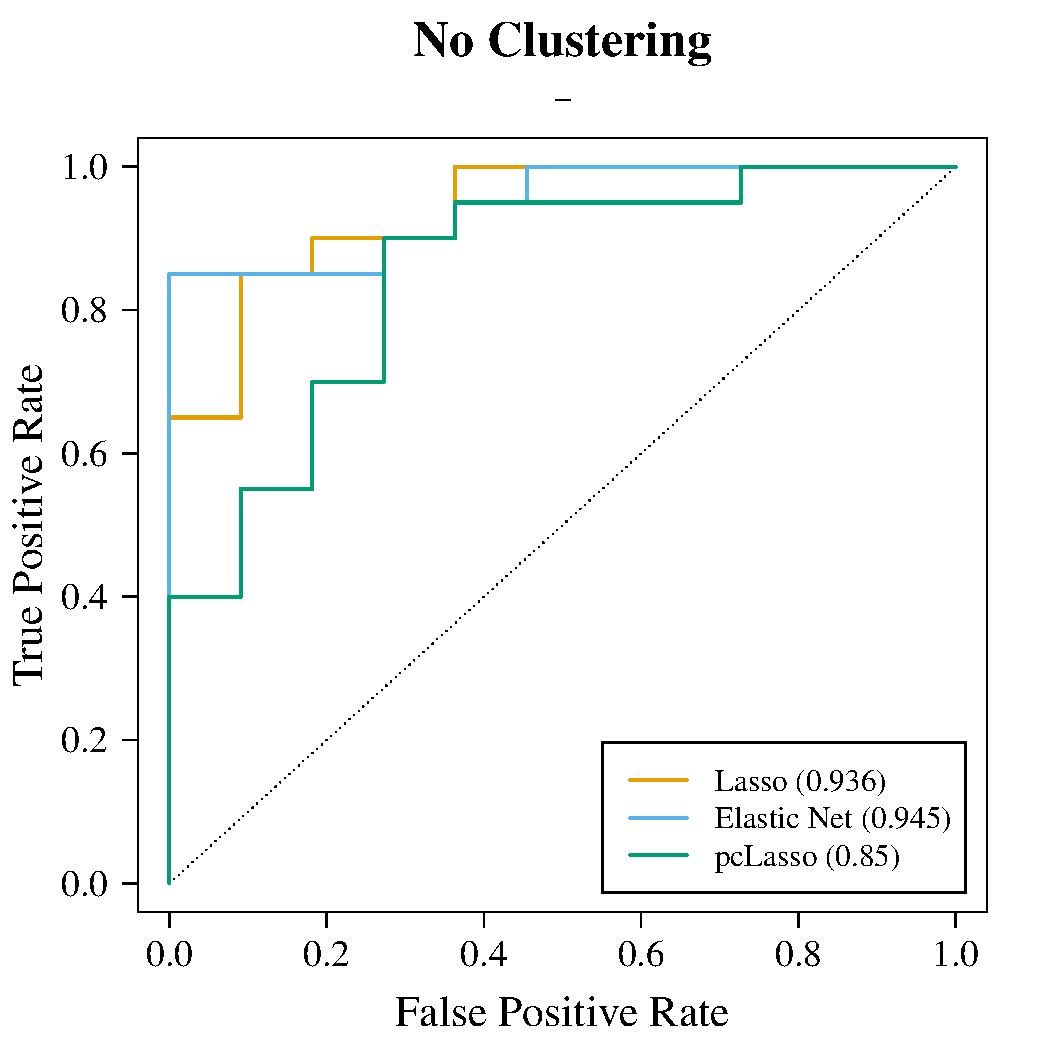
\includegraphics[width = 0.475\textwidth]{colon_ROC_no_n.pdf}
    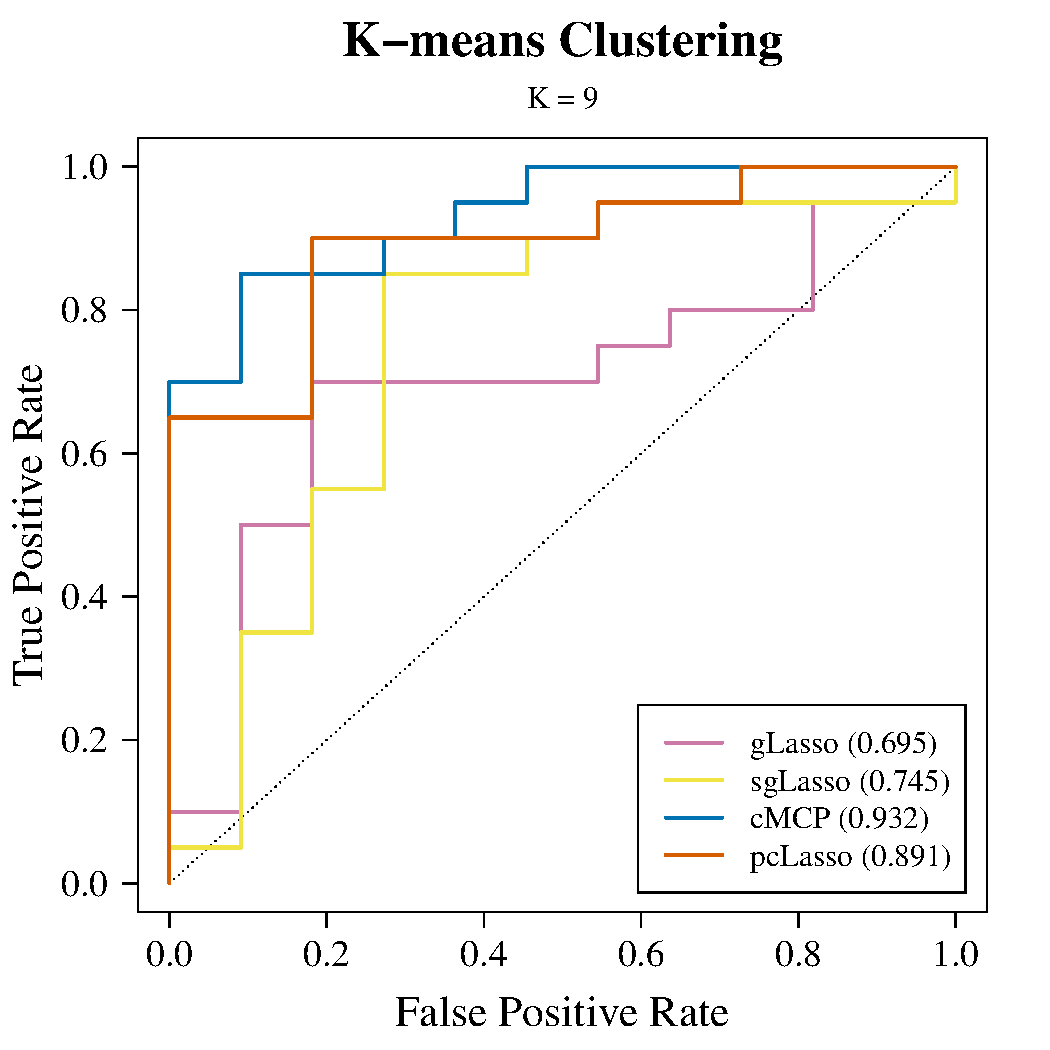
\includegraphics[width = 0.475\textwidth]{colon_ROC_k_n.pdf}
    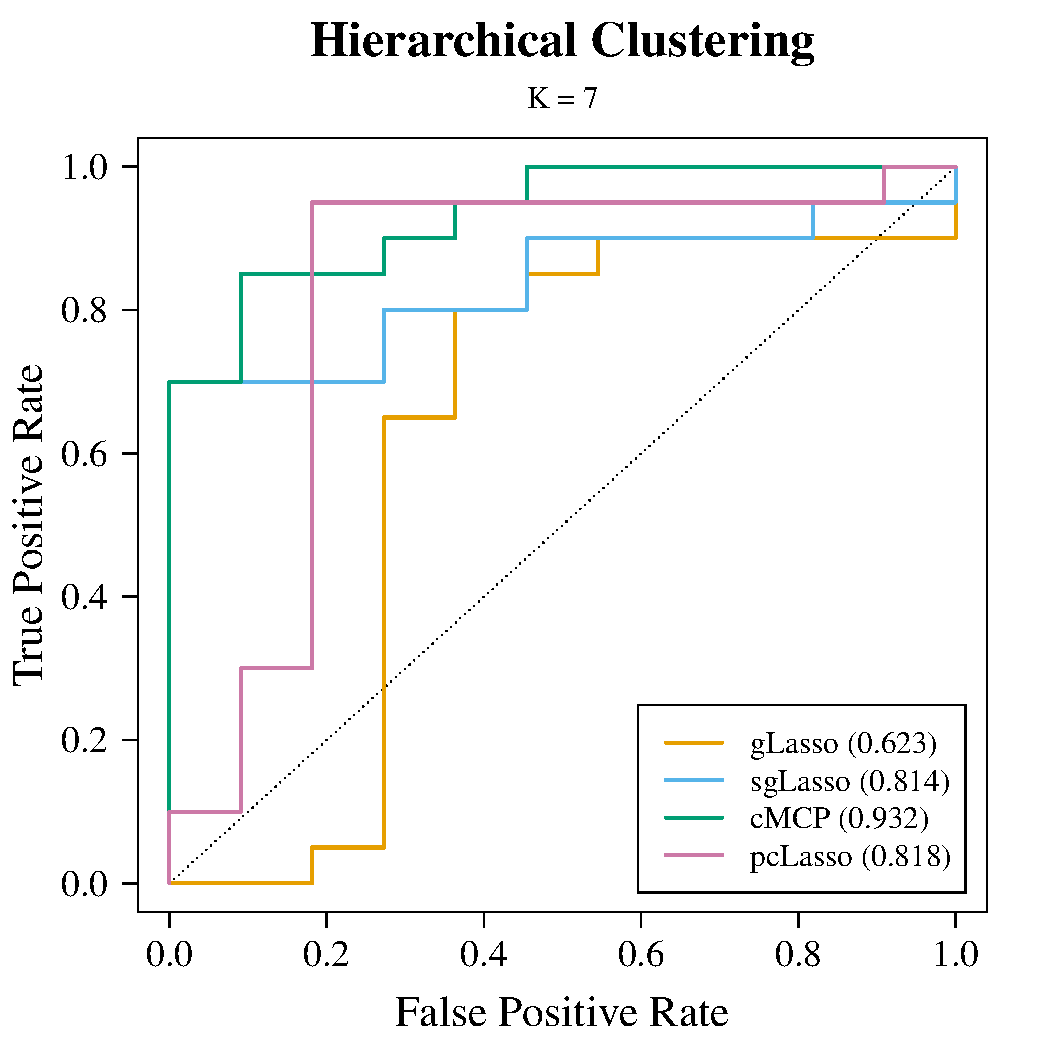
\includegraphics[width = 0.475\textwidth]{colon_ROC_h_n.pdf}
    \caption{The ROC curves for the colon data set.}
    \label{colonROC}
\end{figure}

\end{landscape}
}

We can see that pcLasso using hierarchical clustering performs the best in terms of missclassifications, having only incorrectly predicting 3 of the 31 test observations. When looking at the missclassifications for all of the models, we can see that the lasso, the elastic net, and pcLasso without clustering all perform about the same. 

With $K$-means clustering, gLasso missclassifies 12 of the 31 test observations, which is worse than a null model (the test set had 11 observations that tested negative for cancer and 20 that tested positive). sgLasso performs slightly worse, and cMCP and pcLasso perform about the same as the non-clustered models. Looking at the number of significant groups, we can see that pcLasso does not perform bi-variate selection at all, since all nine groups are represented in the final model. This, along with the poor performance of gLasso and sgLasso, indicate that the grouping structure obtained using $K$-means clustering is not sufficient. 

A similar situation occurs with hierarchical clustering. This time we see that sgLasso missclassifies the most test observations, and gLasso also performs worse than the non-grouped models. Interestingly, the trained cMCP model using hierarchical clustering is identical in size to the model using $K$-means clustering. Finally, pcLasso here both missclassifies the least amount of test observations and has the least number of significant coefficients. There are six significant coefficients (keep in mind the table includes the intercept term) as well as six non-zero coefficients, so again pcLasso does not induce shrinkage at the group level. It is worth noting that pcLasso using hierarchical clustering also has less significant coefficients than all of the non-clustered models, so it is both more accurate and more interpretable. 

\section{Leukemia data set}

The leukemia data set, from \citeay{golub1999molecular}, contains the gene expressions of 7,128 genes for 72 different patients ($n = 72$ and $p = 7,128$). The response is the type of leukemia each patient has; 47 were diagnosed with acute lymphoblastic leukemia (ALL) while 25 were diagnosed with acute myeloid leukemia (AML). 

\subsection{Clustering information}

\begin{figure}[ht]
    \centering
    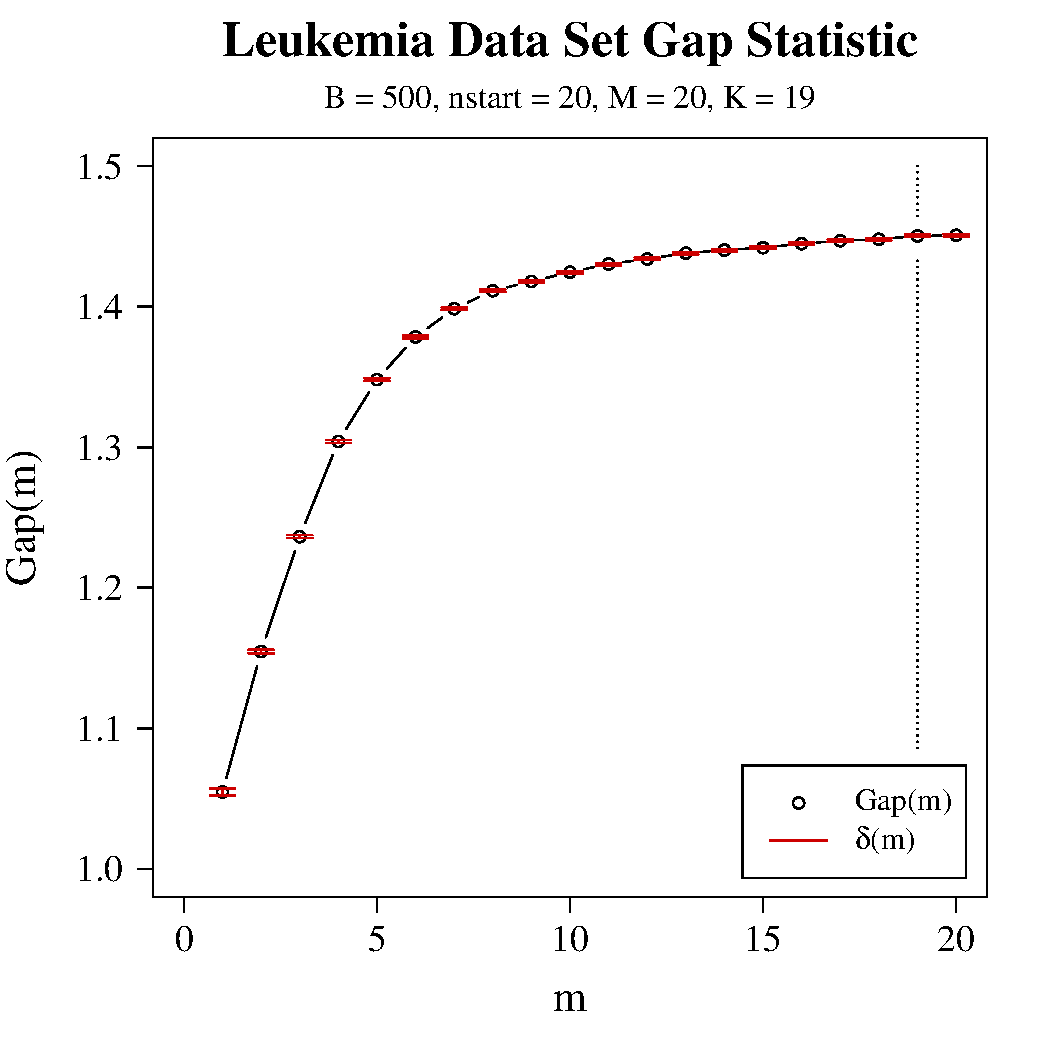
\includegraphics[width = 0.475\textwidth]{leuk_gap_stat.pdf}
    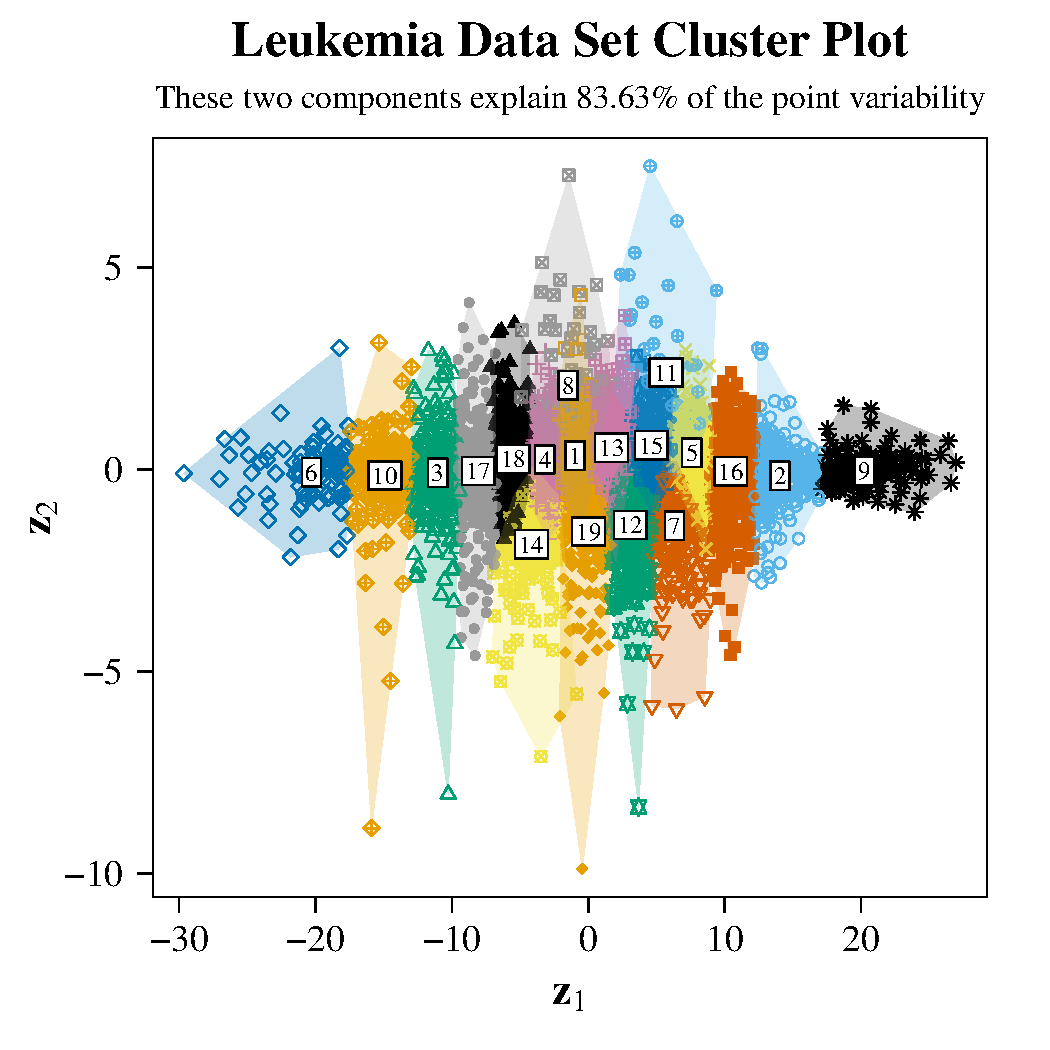
\includegraphics[width = 0.475\textwidth]{leuk_clus_plot.pdf}
    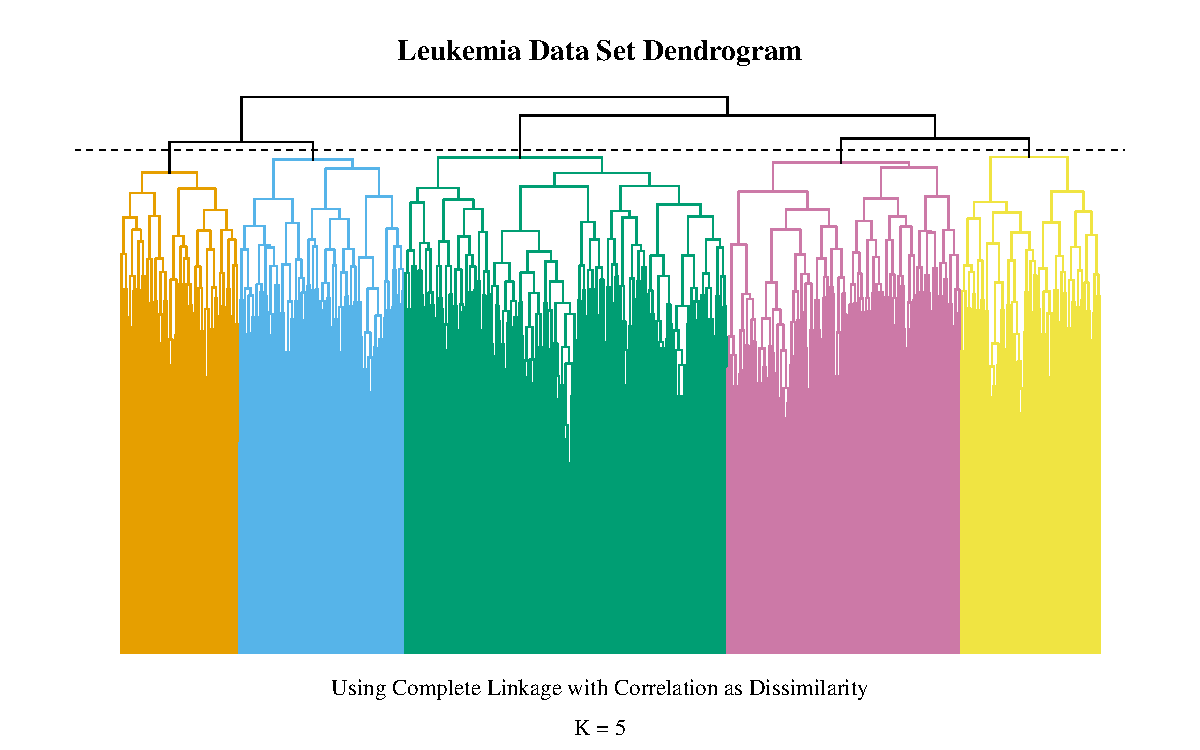
\includegraphics[width = 0.95\textwidth]{leuk_den.pdf}
    \caption{Clustering information for the leukemia data set.}
    \label{leukclus}
\end{figure}

The clustering information for the leukemia data set has been printed in Figure \ref{leukclus}. The gap statistics for $m = 1, \ldots, 20$ have been printed in the top left panel, and $K = 19$ is chosen as the optimal number of clusters. The top right panels plots the predictors against the first two principal components of the observation space, with each group labeled. Finally, the bottom panel shows the leukemia dendrogram; we chose $K = 5$ at the optimal number of clusters. 

\subsection{Results}

\afterpage{
\begin{landscape}
\begin{table}[p]
    \footnotesize
    \centering
    \def\arraystretch{1.5}

    \begin{tabularx}{0.977\linewidth}{lccccccccccc} \toprule
         & \multicolumn{3}{c}{No Clustering} & \multicolumn{4}{c}{$K$-means Clustering} & \multicolumn{4}{c}{Hierarchical Clustering} \\ 
         & \multicolumn{3}{c}{--} & \multicolumn{4}{c}{$K=19$} & \multicolumn{4}{c}{$K=5$} \\   
         \cmidrule(r){2-4} \cmidrule(lr){5-8} \cmidrule(l){9-12}
         % this is what has to be replaced with xtable
         & Lasso & Elastic Net & pcLasso & gLasso & sgLasso & cMCP & pcLasso & gLasso & sgLasso & cMCP & pcLasso \\ \midrule
        \multirow{2}{*}{Parameters} & $\lambda = 0.00407$ & $\lambda = 0.00509$ & $\lambda = 0.00548$ & $\lambda = 0.0779$ & $\lambda = 0.0457$ & $\lambda = 0.111$ & $\lambda = 0.00548$ & $\lambda = 0.0779$ & $\lambda = 0.0236$ & $\lambda = 0.111$ & $\lambda = 0.00548$ \\ 
        & -- &  $\alpha = 0.8$ & $\texttt{rat} = 0.95$ & -- & $\alpha = 0.95$ & $\gamma = 30$ & $\texttt{rat} = 0.9$ & -- & $\alpha = 0.4$ & $\gamma = 30$ & $\texttt{rat} = 0.95$ \\ 
        Deviance & 0.241 & 0.0834 & 0.465 & 1.240 & 0.730 & 0.671 & 0.442 & 1.240 & 0.731 & 0.671 & 0.439 \\ 
        Misclass. & 5/36 & 3/36 & 3/36 & 14/36 & 13/36 & 6/36 & 2/36 & 14/36 & 14/36 & 6/36 & 2/36 \\ 
        Sig. Coef. &  14 &  28 &  41 &   1 &   6 &   6 &  76 &   1 & 772 &   7 &  46 \\ 
        Sig. Groups & -- & -- & -- &  0 &  1 &  2 & 19 &  0 &  1 &  2 &  5 \\ 
        %FPR & 5/14 & 3/14 & 3/14 & 14/14 & 13/14 & 6/14 & 2/14 & 14/14 & 14/14 & 6/14 & 2/14 \\ 
        %TPR & 22/22 & 22/22 & 22/22 & 22/22 & 22/22 & 22/22 & 22/22 & 22/22 & 22/22 & 22/22 & 22/22 \\ 
        AUC & 0.987 & 1.000 & 0.977 & 0.500 & 0.994 & 0.964 & 0.994 & 0.500 & 0.990 & 0.968 & 1.000 \\ 
        %
        \bottomrule
    \end{tabularx}
    \caption{The performance of various models on the leukemia data set.}
    \label{leuktab}

\end{table}

\vspace{0.5cm}

\begin{figure}[p]
    \centering
    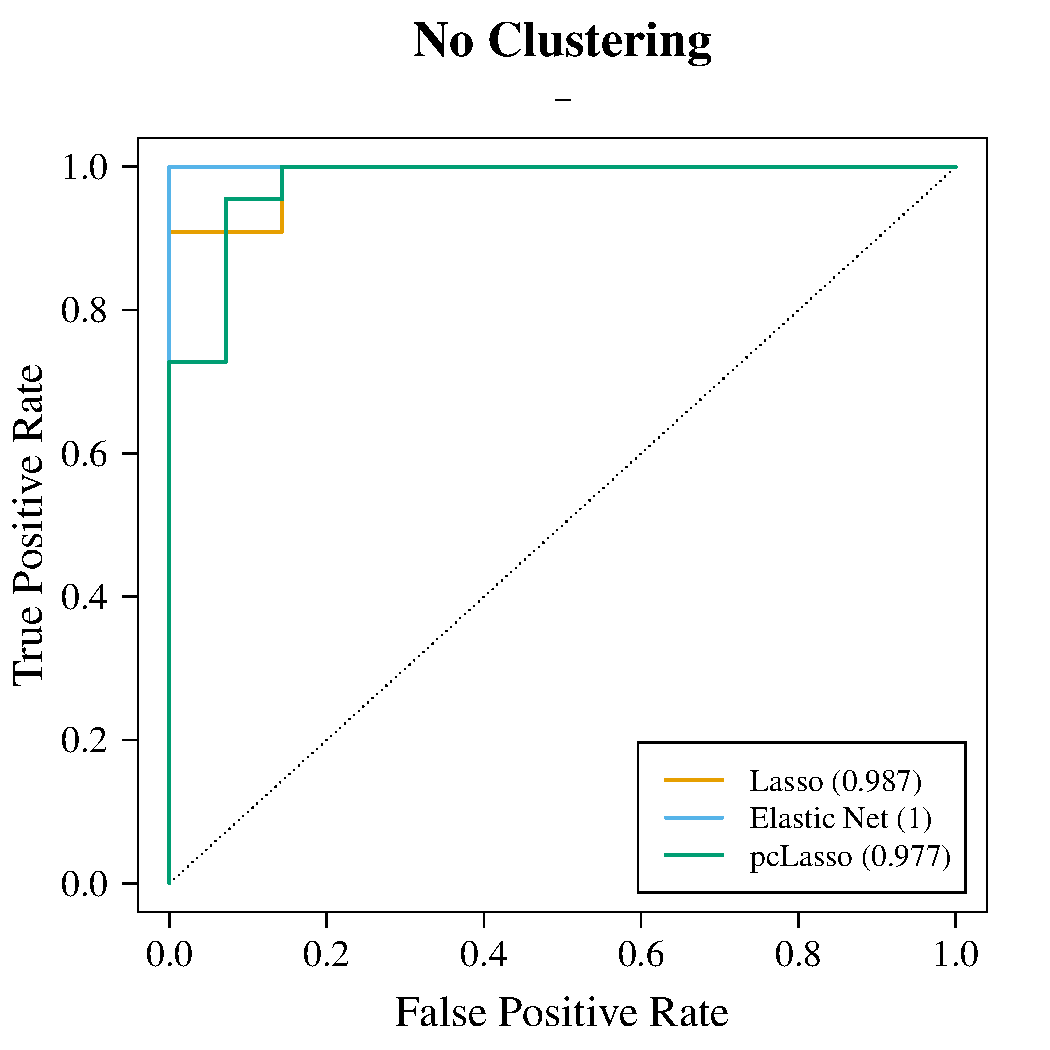
\includegraphics[width = 0.475\textwidth]{leuk_ROC_no_n.pdf}
    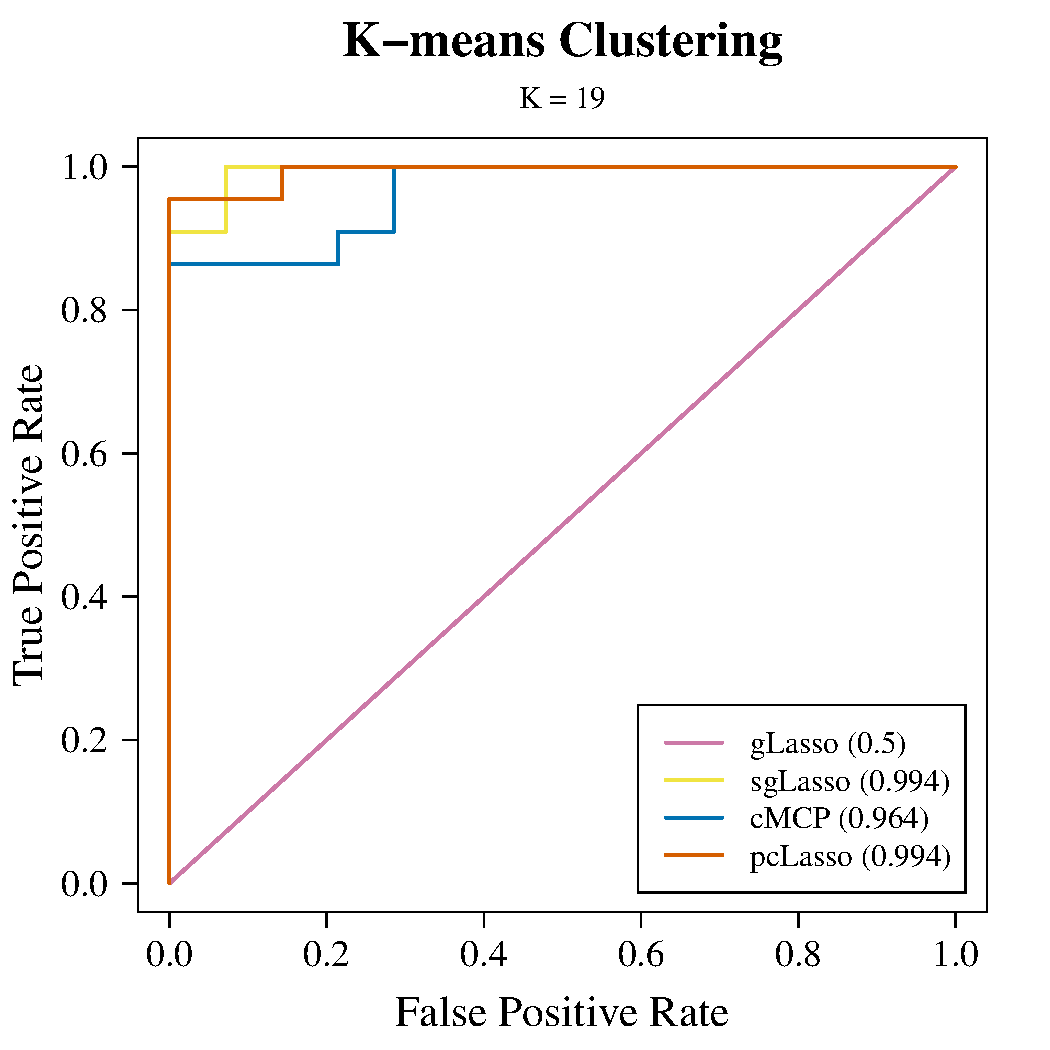
\includegraphics[width = 0.475\textwidth]{leuk_ROC_k_n.pdf}
    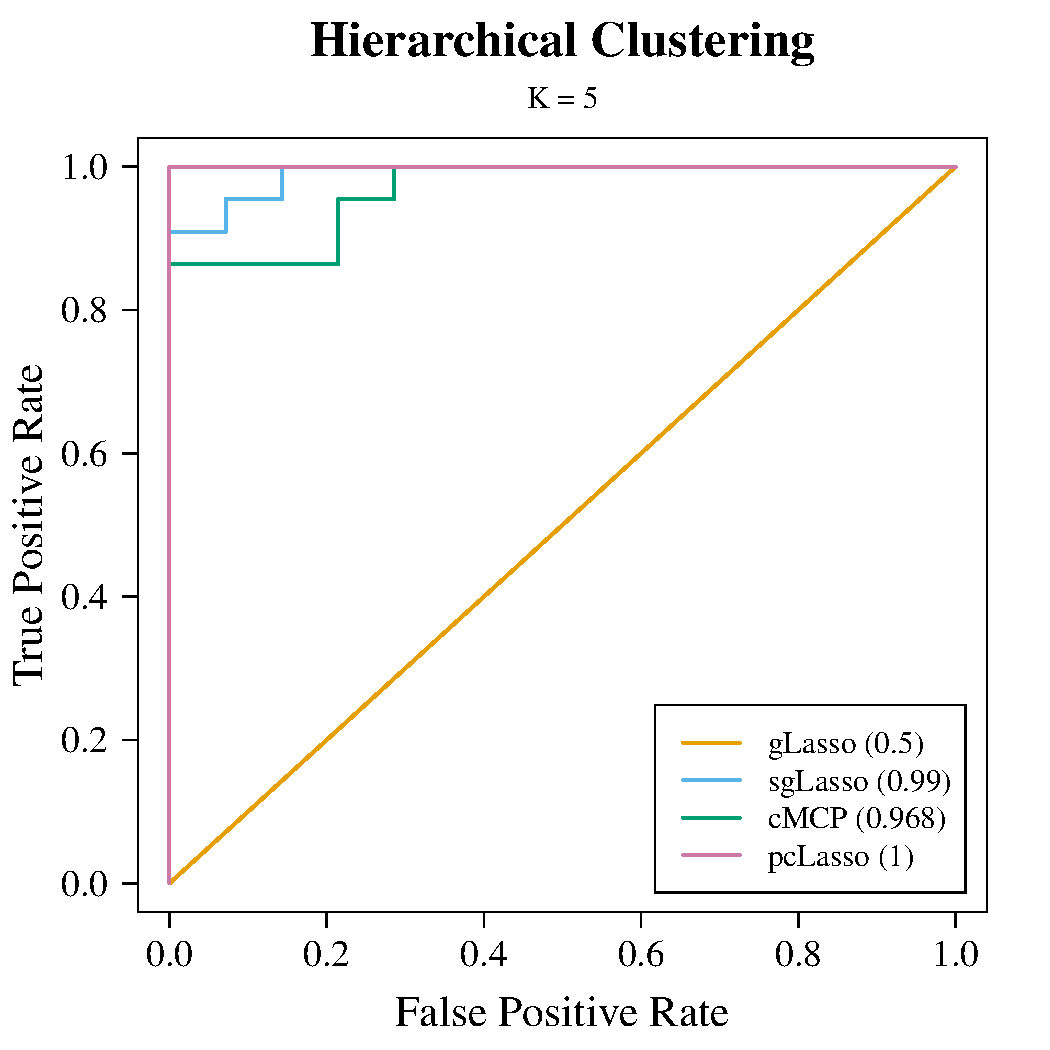
\includegraphics[width = 0.475\textwidth]{leuk_ROC_h_n.pdf}
    \caption{The ROC curves for the leukemia data set.}
    \label{leukROC}
\end{figure}

\end{landscape}
}

The same general set up for the colon data set was applied to the leukemia data set; the results have been printed in Table \ref{leuktab} and the ROC curves have been printed in Figure \ref{leukROC}. As with the colon data set, it seems that the clustering algorithms are unable to identify a sufficient grouping structure. 

For the non-clustered models, both the elastic net and pcLasso perform the same in terms of missclassifications. However, the elastic net has a markedly lower deviance, less significant coefficients, and a higher AUC, making it a decisively better model in this situation. 

Both gLasso and sgLasso perform extremely poorly for both $K$-means and hierarchical clustering; in fact, gLasso actually fits a null model in both cases. cMCP again fits models with similar sizes in both cases, and while the missclassification rate is much better than gLasso and sgLasso, it still performs worse than the non-clustered models. As with the colon data set, clustered pcLasso is the overall winner, having only missclassified two of the 36 test observations in both cases. In addition, we see that pcLasso does not induce shrinkage at the group level. And while both models perform the same in prediction accuracy, pcLasso using hierarchical clustering has a slightly lower deviance, significantly less significant predictors, and a slightly higher AUC, so it can be considered the best model for all of the clustered predictors. 

Unlike the colon data set, however, there is some type of trade-off that one would have to consider when choosing an overall best model. While pcLasso with hierarchical clustering has the lowest number of missclassifcations, it has 45 significant predictors. On the other hand, the lasso and the elastic net have 13 and 27, respectively, so even though their missclassification rates are slightly higher, they are more interpretable models. It is entirely reasonable for one to choose a model with one additional incorrect prediction if it is easier to interpret and explain. 

\section{Discussion}

With both data sets, we saw that the group lasso and the sparse group lasso performed very poorly relative to the other methods, especially for the leukemia data set. In addition, pcLasso did not perform bi-variate selection. Both of these facts are indications that both $K$-means clustering and hierarchical clustering were \textit{ineffective} in properly identifying a grouping structure that was relevant to the response. However, we also observed that pcLasso with clustered predictors had a slighlty lower number of missclassifications than the non-clustered models, showing that even though the groups were not relevant to the response, the models can potentially become more accurate and interpretable. 

There are several avenues that one could follow for further research:
\begin{itemize}
    \item Looking at the top right panels of Figures \ref{colonclus} and \ref{leukclus}, we can see that the clusters are not well-separated at all. Despite this, the gap statistic split the predictors into a rather large number of clusters, especially for the leukemia data set, which may be a result of the large number of predictors. Perhaps another measure to determine the optimal number of clusters can be used. It is also worth mentioning that the computation time when using the \texttt{clusGap} function was on the magnitude of \textit{hours}, making it non-practical for larger data sets.
    \item The two clustering algorithms used were chosen because of their simplicity and reputation, but one could argue that their poor performance is entirely expected. Much work has been done in the field of unsupervised learning, and one could use a different clustering algorithm to generate the group structure.
    \item There are many more grouped regularization models that can be employed that perform bi-variate selection, such as the group exponential lasso (``GEL'') \cite{Breheny2015TheGE} or the group bridge \cite{huang2009group}, that can be efficiently implemented using the \texttt{grpreg} package. Each of these methods have their own interesting properties, and one could investigate if their use can improve over the non-clustered models.
\end{itemize}

\textbf{Acknowledgements}: We would like to thank J. Kenneth Tay for his helpful comments about pcLasso and undergraduate research in general. We would also like to thank Patrick Breheny for his helpful comments about his \texttt{grpreg} package. The authors were supported by NSF Award 1757717.

%\newpage
%------------------------------------------------------
%                      References
%------------------------------------------------------

\bibliographystyle{apacite}
\bibliography{report}

%------------------------------------------------------
%                      Appendix
%------------------------------------------------------

%\renewcommand\thesection{\Alph{section}}
%\setcounter{section}{0}

%\section{Information about the GAP statistic} \label{AppA}



%\section{Details on Clustering Methods for Real World Data}

%Here are the dendrograms and stuff blah blah

\end{document}

% https://stats.stackexchange.com/questions/220243/the-proof-of-shrinking-coefficients-using-ridge-regression-through-spectral-dec

% https://stats.stackexchange.com/questions/297280/ridge-regression-increase-in-lambda-leads-to-a-decrease-in-flexibilty/297475#297475

% https://stackoverflow.com/questions/9071020/compute-projection-hat-matrix-via-qr-factorization-svd-and-cholesky-factoriz

% https://www.cs.cornell.edu/courses/cs3220/2010sp/notes/svd.pdf

% https://intoli.com/blog/pca-and-svd/

% https://stats.stackexchange.com/questions/134282/relationship-between-svd-and-pca-how-to-use-svd-to-perform-pca

% https://stats.stackexchange.com/questions/297280/ridge-regression-increase-in-lambda-leads-to-a-decrease-in-flexibilty/297475#297475

% https://stats.stackexchange.com/questions/147880/is-pca-still-done-via-the-eigendecomposition-of-the-covariance-matrix-when-dimen